\chapter{Einleitung}

In der Einleitung werden die Systemkomponenten der Arbeit erläutert. Dadurch erhält man einen Überblick wie das Aufnahmesystem mit dem Server zusammenspielt. Für das Verständnis wird das Aufgabenumfeld in einem abstrakten Kontext dargestellt. Die konkrete Implementierung und detailierte Analyse werden dann in den folgenden Kapitel behandelt.

\section{Big Picture}
Zur Übersicht werden die verschiedenen Komponenten des Projektes in einem Big Picture zusammengefasst. Die Grafik \ref{fig:bigpicture} ist in drei Abschnitte unterteilt. Im obersten Abschnitt befinden sich alle Geräte, welche Daten erfassen. Diese Aufnahmesysteme bestehen aus der Android TourLiveApp, als Teil dieser Arbeit, sowie dem Android RadioTourSpeaker welcher im Rahmen einer anderen Arbeit entwickelt wurde.\\
Im mittleren Teil befinden sich die Serversysteme. Diese besteht aus einem TourLive Server, welcher die Renndaten empfängt und verarbeitet sowie dem Geräteverwaltungsserver. Der Geräteverwaltungsserver bietet eine Übersicht über die registrierten Aufnahmesysteme und ermöglicht es deren Einstellungen zu Verwalten sowie allfällige Fehlerquellen frühzeitig zu erkennen.\\
Der unterste Abschnitt zeigt die Anwendergruppen, die mit den Daten beliefert werden. Dies sind zum einen die Besucher der Webseite, welche in dieser Arbeit umgesetzt wurde, sowie auch Drittentwickler, die Interesse an diesen Daten haben.\\
Teil dieser Arbeit sind die farblich hervorgehobenen Komponenten: Die Aufnahmesysteme TourLiveApp in Form einer Android App [rot], das Serversystem TourLive Server in Form einer Spring Webapplikation [blau] sowie das Serversystem Device Management Server ebenfalls in Form einer Spring Webapplikation [grün].

\begin{figure}[H]
	\centering
	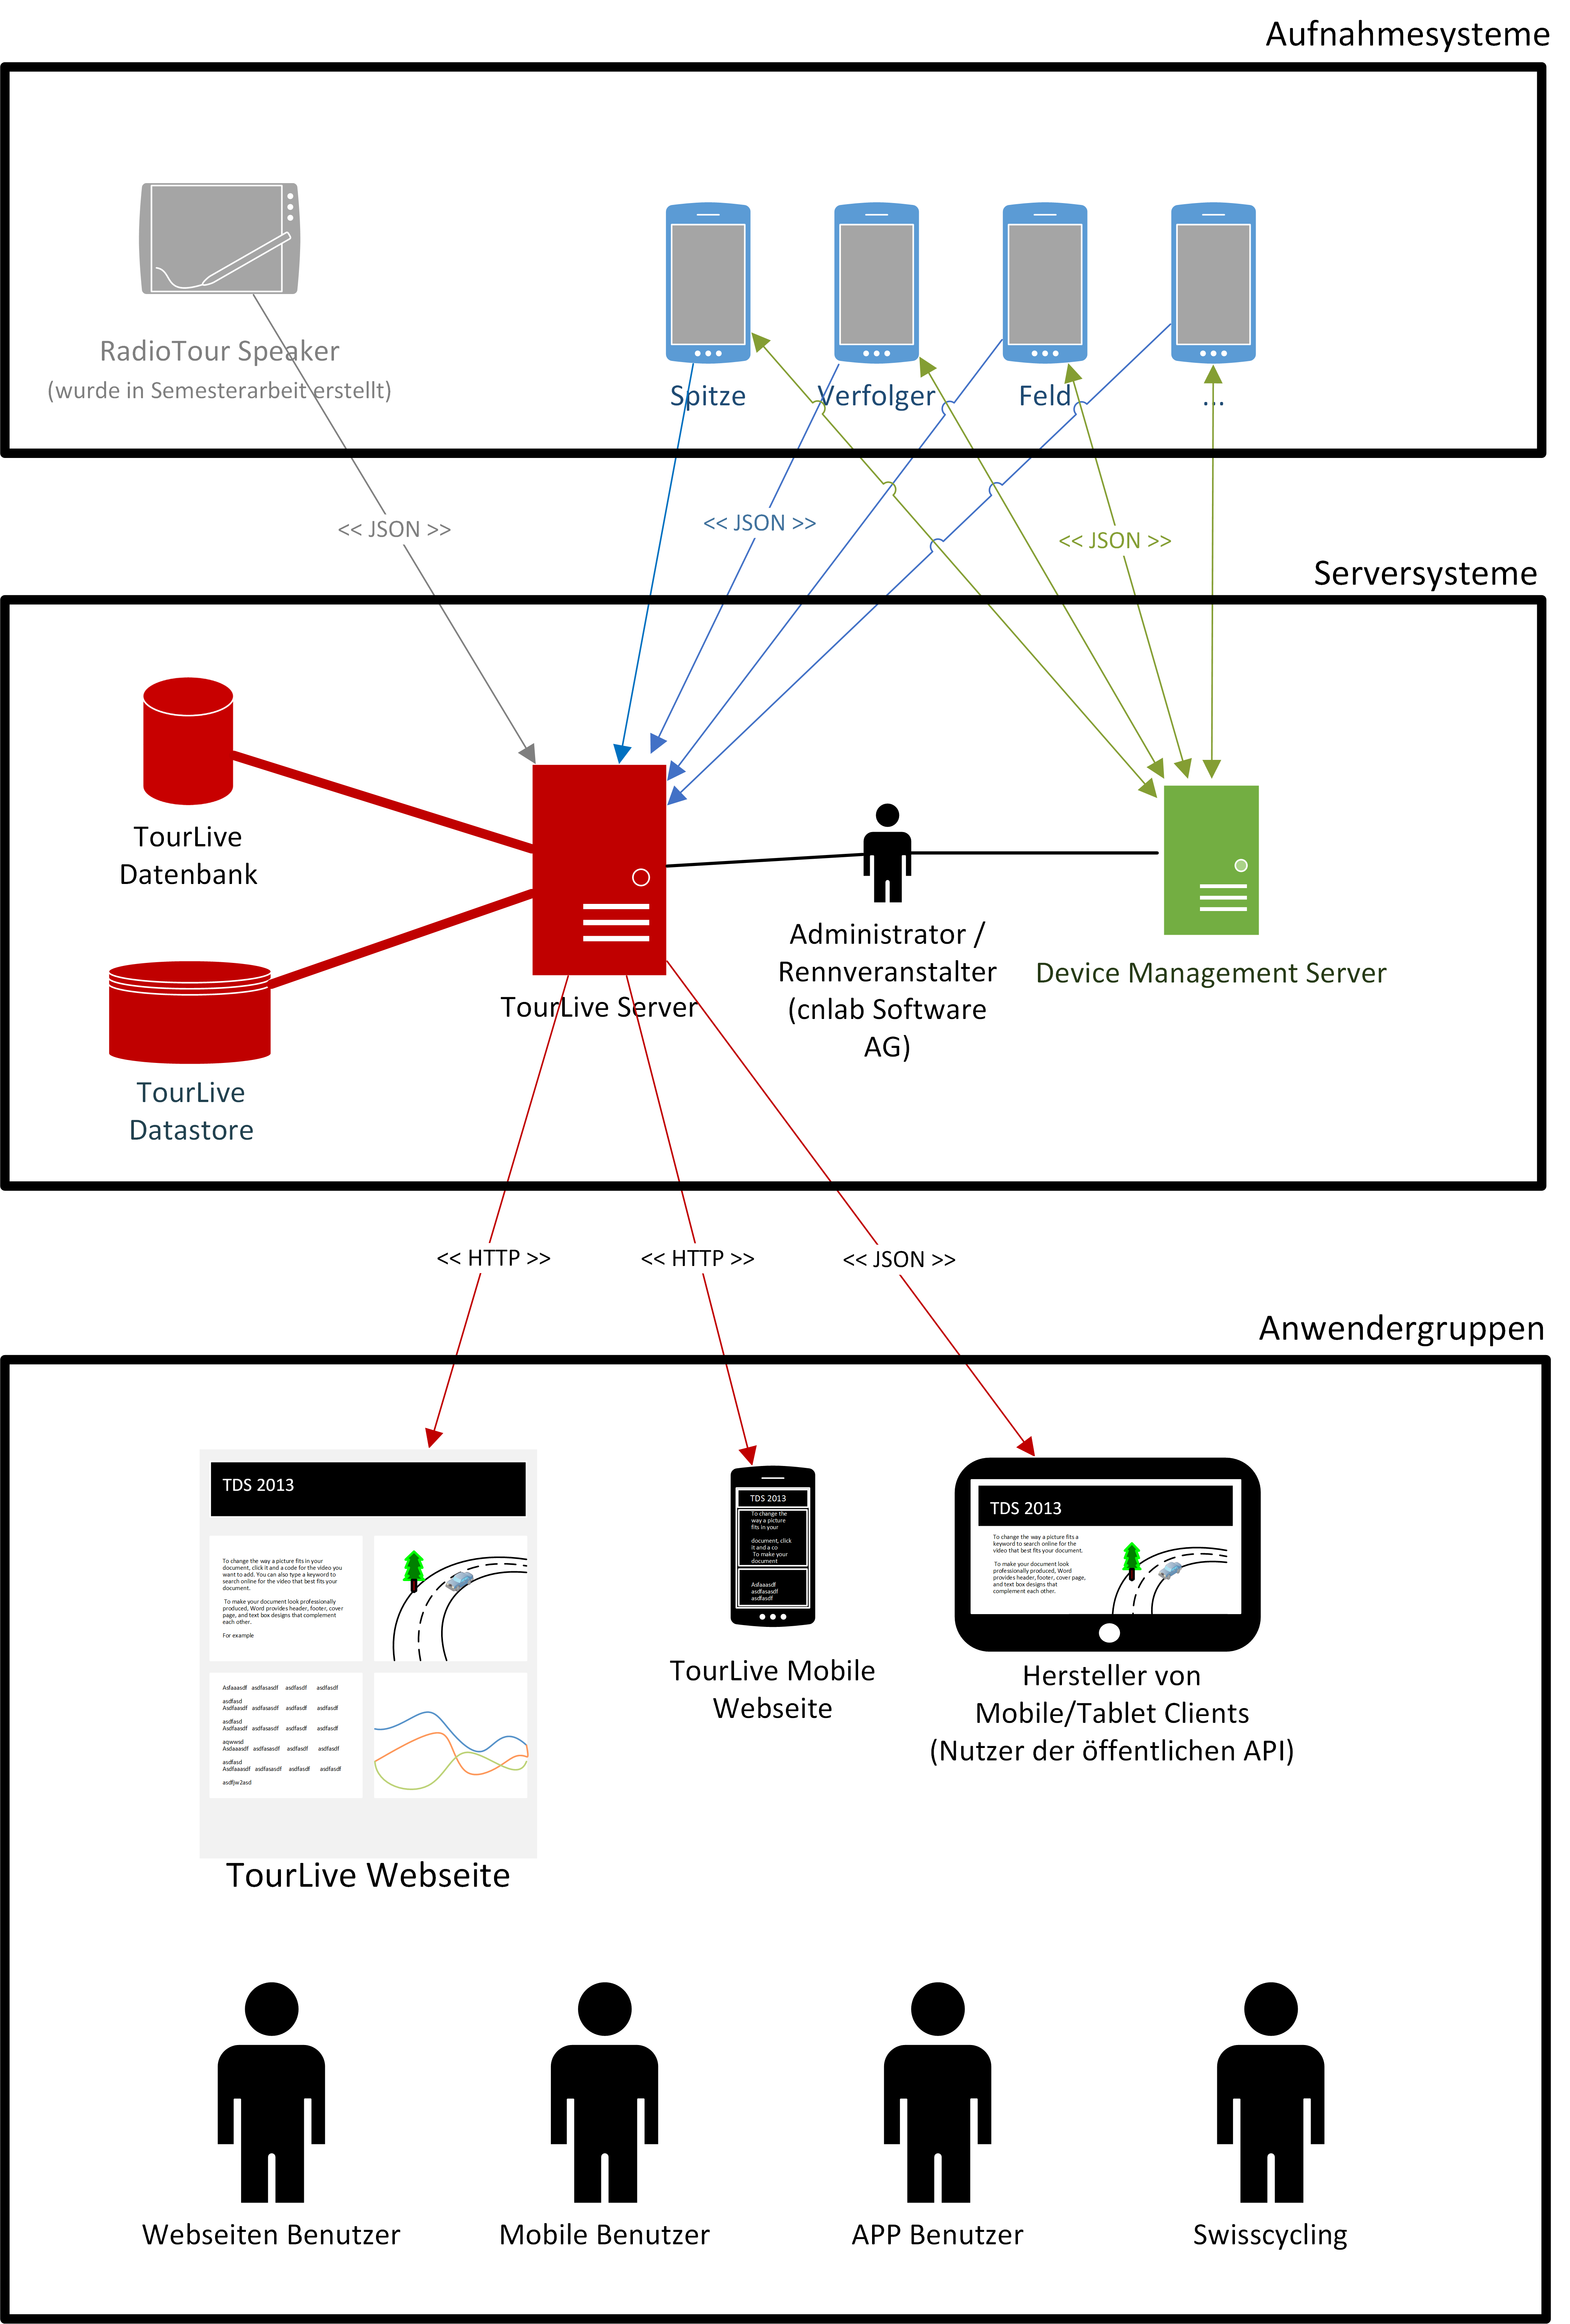
\includegraphics[height=200mm]{images/BigPicture.png}
	\caption{BigPicture}
	\label{fig:bigpicture}
\end{figure}

\pagebreak

\section{Kernelemente}
Die drei oben erwähnten Kernsysteme werden im folgenden kurz beschrieben.

\subsection{TourLive Server}
Auf der zentralen Webapplikation TourLive Server werden die eingehenden Daten von den Aufnahmesystemen gespeichert, verarbeitet, aufbereitet und weitergegeben. Bild und Positionsdaten werden in Form einer Webseite für Radsportbegeisterte aufbereitet und für mögliche Drittentwickler zur Verfügung gestellt. Die Architektur wurde dabei so gewählt, dass das System bei hoher Last gut skaliert. Diese Komponente wird im Kapitel \ref{sec:tourliveserver} genauer behandelt.

\subsection{Device Management Server}
Der Device Management Server hilft dabei, die aktiven Aufnahmegeräte zu verwalten. Es ersetzt das existierende Portal, dass nur wenig Funktionalität besitzt. Sollte der Device Management Server nicht verfügbar sein, sind die Aufnahmegeräte trotzdem einsatzfähig, da die Einstellungen lokal am Smartphone gesetzt werden können.

\subsection{Aufnahmesystem}
Ein wesentlicher Bestandteil des Endsystems ist das Aufnahmesystem. Es ersetzt die Symbian App auf den Nokia Handys. In der folgenden Abbildung sieht man links das Aufnahmesystem, welches von den Satelliten GPS Daten empfängt. Periodisch werden alle gesammelten Daten vom Aufnahmesystem an den TourLive Server übermittelt. Ebenfalls periodisch werden die Einstellungen vom Device Management Server abgeholt. Werden die Einstellungen lokal verändert so werden die veränderten Einstellungen an den Device Management Server übertragen.


\section{Aufgabenaufteilung}
{\renewcommand{\arraystretch}{2}%
    \begin{longtable}{  p{7.0cm} | p{4.0cm} }
    \textbf{Komponente} & \textbf{Bearbeitet durch} \\ 
  	\hline
	\hline
    TourLive Server & Florian Bentele \\
    \hline
    TourLiveApp & Patrizia Heer\newline Simon Stäheli \\
    \hline
    Device Management Server & Patrizia Heer \newline Simon Stäheli \\
    \hline
\caption{Aufgabenaufteilung}
\end{longtable}}
